\documentclass[../../lecture_notes.tex]{subfiles}

\begin{document}

\noindent Constraint Satisfaction Problems are a subclass of problems where
\begin{itemize} [itemsep=0mm]
	\item the path to the solution is not relevant
	\item the state space is sufficiently large
\end{itemize} \medskip

\noindent We solve these problems by breaking up the state space into smaller atomic elements.\\

A constraint satisfaction consists of a few parts:
\begin{enumerate} [itemsep=0mm]
	\item variables {$X_1, ... X_n$}
	\item domain {$D_1, ..., D_n$} of values for each X to be assigned
	\item constraints {$X_iD_i$ | consistent assignments}
\end{enumerate} \medskip

\noindent Consider a state map of Australia:

\begin{figure} [H]
	\centering
	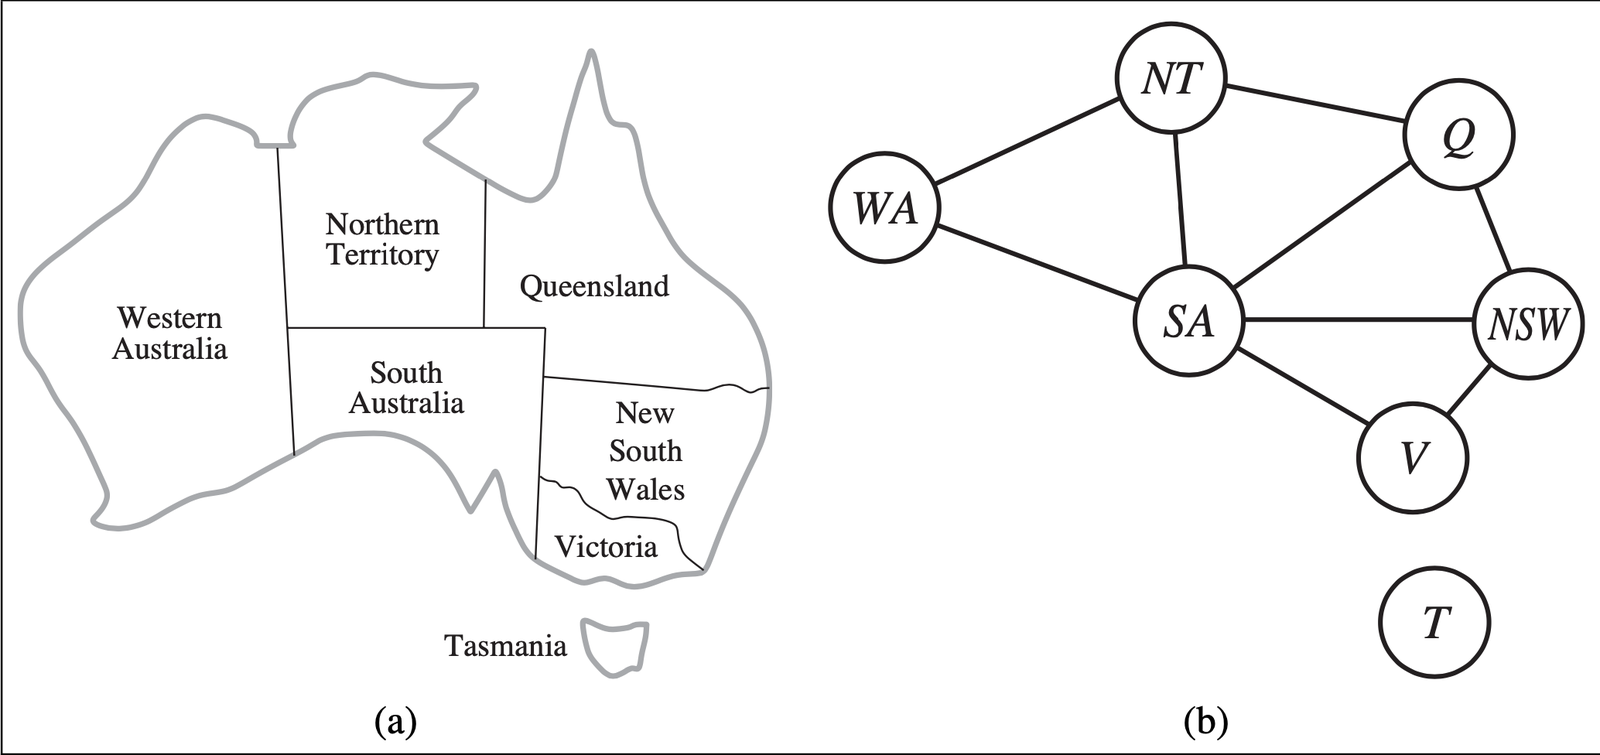
\includegraphics[width=0.8\textwidth]{AU}
\end{figure}

\noindent We wish to color the map in 3 colors such that adjacent states differ in color.\\
\indent \{X\} = \{WA, NT, NSW, V, SA, T\}\\
\indent D = \{R, G, B\}\\
\indent WA != ST...\\
We can visualize this problem using a constraint graph, since constraints are binary.\\
This is as opposed to unary constraints (single element rules).\\
The Rules:
\begin{enumerate} [itemsep=0mm]
	\item each variable forms a node
	\item each constraint forms an edge
\end{enumerate} \medskip

\noindent Constraint Satisfaction Problems seem specific, but the algorithms end up very generalizable.\\
 There are two categories of problems
 \begin{enumerate} [itemsep=0mm]
	\item \textbf{\underline{Hard CSP}} $\equiv$ no violation of constraints allowed
	\item \textbf{\underline{Soft CSP}} $\equiv$ some constraints are preference constraints and not required.\\
                (These are also called constraint optimization problems)
\end{enumerate} \medskip

\noindent There is one major form of problem where contests are held for who can solve it the best:

\subsection*{Satisfiability (SAT)}
	Variables: ${X_1, X_2, ..., X_n}$\\
	Values: ${1, 0}$\\
	Constraints: $\{X_1 \lor \neg X_2 \lor X_4, X_2 \lor \neg X_3 \lor X_5, ...\}$\\
\\
This was the first and is now the prototypical NP-Complete problem!\\
\textbf{\underline{Complete}}:
	\begin{itemize} [itemsep=0mm]
		\item the “hardest” problem in a given complexity class
		\item if you can provide a solution, you can solve all problems in the class
	\end{itemize}
	
\subsection*{Formulating CSP as Search}
\noindent Let’s walk through an example tree w/ var = ${x, y, z}$ \& $D = {0, 1}$:\\

\begin{center} \begin{tikzpicture}
	\node {}
	child {node[ellipse, draw] {x=0}
		child {node{}
			edge from parent node {}}
		child {node{}
			edge from parent node {}}
		child {node{}
			edge from parent node {}}
		child {node[ellipse, draw]  {z=1}
			child {node {}
				edge from parent node {}}
			child{node [rectangle, draw] {x=0, y=1, z=1}
					edge from parent node[right] {}}
			edge from parent node [right] {}}
		edge from parent node [left] {}}
	child {node{}
		edge from parent node {}}
	child {node{}
		edge from parent node {}}
	child {node{}
		edge from parent node {}}
	child {node{}
		edge from parent node {}}
	child {node [ellipse, draw] {z=1}
		child {node{}
			edge from parent node {}}
		child {node{}
			edge from parent node {}}
		child {node{}
			edge from parent node {}}
		child {node [ellipse, draw] {y=1}
			child{node [rectangle, draw] {x=0, y=1, z=1}
				edge from parent node [left] {}}
			child {node {}
				edge from parent node {}}
			edge from parent node [right] {}}
		edge from parent node [right] {}};
\end{tikzpicture} \end{center}
\noindent This is terrible and would be unfeasible; luckily we can note there are only 8 complete states!\\
$\implies$ If we let nodes be variables and edges values with DFS, we get time $O(d^n)$ \& space $O(dn)$.\\
\\
A straight BFS may not be optimal, however, as we may violate constraints early;\\
	\indent thus we backtrack, failure testing at intermediate nodes.\\

\noindent We can improve the efficiency of backtracking by answering a few questions:
\begin{enumerate} [itemsep=0mm]
	\item Which variable do we assign next?
	\item Which value should we try next?
	\item Can we detect failure early?
	\item Can we take advantage of the problem structure?
\end{enumerate}

\subsection*{Variable \& Value Ordering}
\noindent Consider the following problem:\\
	\indent Variables: ${x, y, z}$\\
	\indent Values: ${0, 1}$\\
	\indent Constraints: ${x=y, y=z}$\\
\begin{center} \begin{tikzpicture}
\node [text width=4cm] (L) { \begin{forest} [X [Y [Z  [(+)]  [(-)]] [Z  [(-)] [(-)]]] [Y[Z [(-)] [(-)]][Z [(-)] [(+)]]]] \end{forest}};
\node [text width=4cm, right =3cm of L] (R) { \begin{forest} [X [Y [Z  [(+)]]] [Y [Z [(+)]]]] \end{forest}};
\draw [->] (L.north east) -- node [align=center, above] {condenses to} (R.north west);
\end{tikzpicture} \end{center}

\noindent Note that if we use the tree to the left, we must search the entire tree.\\
If we reorder the variables, however, we can prune the tree and use the right tree.\\
\\
When it comes to ordering,\\
	\indent \textit{Variable} ordering changes branch count.\\
	\indent \textit{Value} ordering changes branch order.\\
We can choose variables and values based on a few models:
\begin{enumerate} [itemsep=0mm]
	\item \textbf{\underline{Most Constrained Variable}}
		 $\equiv$ choose the variable with the minimum remaining values
	\item \textbf{\underline{Most Constraining Variable}} 
		$\equiv$ choose the variable that places the most constraints
	\item \textbf{\underline{Least Constraining Value}}
		$\equiv$ choose the value that places the least restrictions
\end{enumerate}

\noindent We choose this model heuristically via direct time comparison.\\
\\
This leads us toward our methods of early failure detection\\
	\indent Forward Checking -- less effective but more efficient\\
	\indent Arc Consistency -- more effective but less efficient

\subsection*{Forward Checking}
$\equiv$ keep track of the consistent values unassigned variable; if a variable has no values left, then failure!

\begin{center} \begin{tikzpicture}
	\node [circle, draw] (WA) {WA};
	\node [circle, draw, above right =of WA] (NT) {NT};
	\node [circle, draw, below right =of WA] (SA) {SA};
	\node [circle, draw, above right =3cm of SA] (Q) {Q};
	\node [circle, draw, below right =of Q] (NSW) {NSW};
	\node [circle, draw, below left =of NSW] (V) {V};
	\node [circle, draw, below right =of V] (T) {T};
	\draw [-] (WA.north east) -- (NT.south west);
	\draw [-] (SA.north west) -- (WA.south east);
	\draw [-] (SA.north) -- (NT.south);
	\draw [-] (NT.east) -- (Q.north west);
	\draw [-] (SA.north east) -- (Q.south west);
	\draw [-] (SA.north east) -- (NSW.west);
	\draw [-] (SA.east) -- (V.west);
	\draw [-] (Q.south east) -- (NSW.north);
	\draw [-] (NSW.south west) -- (V.east);
	\node [align=center, below =6cm of NT] (3) {Q\\R(G)B};
	\node [align=center, left =of 3] (2) {NT\\\sout{RG}B};
	\node [align=center, left=of 2] (1) {WA\\(R)GB};
	\node [align=center, right =of 3] (4) {NSW\\R\sout{GB}};
	\node [align=center, right =of 4] (5) {V\\RG(B)};
	\node [align=center, right =of 5] (6) {SA\\\sout{RGB}};
	\node [align=center, right =of 6] (7) {T\\RGB};
\end{tikzpicture} \end{center}
\subsection*{Arc Consistency}
$\equiv$ make all arcs consistent; if we can, then assign arbitrarily left to right, else fail.\\
An arc is \textbf{\underline{consistent}} if for all values of x, there exists a corresponding value of y;\\
	\indent we can therefore propagate constraints across the arc from the right.\\

\begin{center} \begin{tikzpicture}
	\node [circle, draw, align=center] (V) {V\\RGB};
	\node [circle, draw, align=center, right =of V] (NSW) {NSW\\RB};
	\node [circle, draw, align=center, right =of NSW] (SA) {SA\\RGB};
	\draw [-] (V.east) -- node [align=center, above] {+}  (NSW.west);
	\draw [-] (NSW.east) -- node [align=center, above] {+} (SA.west);
	\node [below=of NSW, align=center] (txt) {This arc is \textbf{\underline{consistent}}};
	\node [circle, draw, align=center, below =of txt] (5) {NSW\\R};
	\node [circle, draw, align=center, left =of 5] (4) {V\\RGB};
	\node [circle, draw, align=center, right =of 5] (6) {SA\\B};
	\draw [-] (4.east) -- node [align=center, above] {-} (5.west);
	\draw [-] (5.east) -- node [align=center, above] {+} (6.west);
	\node [below=of 5, align=center]{This arc is \textbf{\underline{inconsistent}}};
\end{tikzpicture} \end{center}
\textbf{\underline{ripple effect}} $\equiv$ check an arc when a value is removed.\\
Single ripple effect: $O(d)$\\
\indent \indent A binary CSP arc count: $O(n^2)$\\
\indent \indent \indent Checking consistency of an arc: $O(n^2)$\\
$\implies$ $T = O(n^2d^3)$ for a binary CSP; that is not bad!

\subsection*{Symmetry}

\subsubsection*{Disconnection}
\noindent Consider the AU coloring problem;\\
\indent we know Tanzania is disconnected, so we can assign it a value arbitrarily.\\
As a general rule, we can solve disconnected components of a search problem separately.\\
\\
Consider a search problem with n=80 \& d=2 @ 10 million nodes per second;\\
\indent the time complexity without division is $2^80$ or 4 billion years!\\
\indent breaking the problem into 4 disconnected reduces the time cost to $4*2^20$ = 0.4 seconds!\\

\subsubsection*{Trees}
\noindent Tree structured CSPs are especially simple to solve.\\
Algorithm:
\begin{enumerate} [itemsep=0mm]
	\item Orient the tree
	\item Make arcs consistent
	\item Assign values
\end{enumerate}
We call the resulting structure a \textbf{\underline{backtrack tree}}.\\
Since the arcs are consistent, we can assign any permissible value!\\
\begin{center}\begin{tikzpicture}
	\node [circle, draw] (A) {A};
	\node [circle, draw, below right =of A] (B) {B};
	\node [circle, draw, below left =of B] (C) {C};
	\node [circle, draw, right =of B] (D) {D};
	\node [circle, draw, above right =of D] (E) {E};
	\node [circle, draw, below right =of D] (F) {F};
	\draw [->] (A.south east) -- (B.north west);
	\draw [->] (B.south west) -- (C.north east);
	\draw [->] (B.east) -- (D.west);
	\draw [->] (D.north east) -- (E.south west);
	\draw [->] (D.south east) -- (F.north west);
\end{tikzpicture}\\\bigskip\begin{tikzpicture}
	\node [circle, draw] (A) {A};
	\node [circle, draw, right =of A] (B) {B};
	\node [circle, draw, right =of B] (C) {C};
	\node [circle, draw, right =of C] (D) {D};
	\node [circle, draw, right =of D] (E) {E};
	\node [circle, draw, right =of E] (F) {F};
	\draw [->] (A.east) -- (B.west);
	\draw [->] (B.east) -- (C.west);
	\draw [->] (B.north east) to [out=30, in=150] (D.north west);
	\draw [->] (D.east) -- (E.west);
	\draw [->] (D.north east) to [out=30, in=150] (F.north west);
\end{tikzpicture}\end{center}

\noindent As an addendum, we can introduce symmetry via a constraint (such as x < y < z);\\
\indent this greatly constricts the problem size, BUT deleting all symmetry is NP-Hard!

\end{document}